\subsection{Spherical Space DA with Pseudo-label Loss}

Now we are going to the next article \textit{"Spherical Space Domain Adaptation with Robust Pseudo-label Loss"} written by  Xiang Gu, Jian Sun, and Zongben Xu. \cite{gu2020spherical} The authors propose a spherical space representation of data, which allows them to get more effective feature extraction and better adaptation across domains. One approach associated with increasing performance with differences in data distribution between source and target domain is to use pseudo-labels. However, the use of pseudo-labels can be problematic in the presence of noisy or incorrect labels. To tackle this problem, the authors map the data to a high-dimensional sphere and introduce a new loss function, called the robust pseudo-label loss, which is designed to address the problem of noisy or incorrect labels in the target domain. 

\begin{figure}[H]
    \centering
    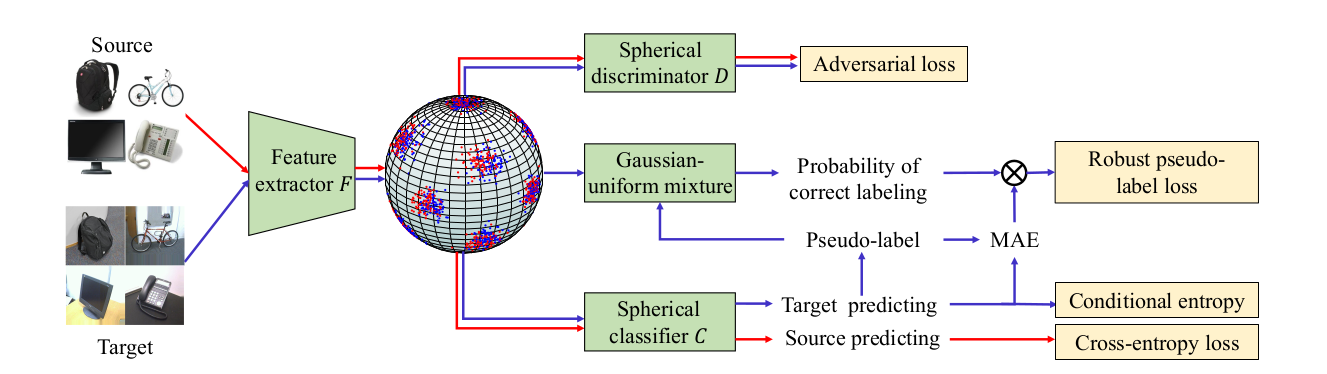
\includegraphics[width=\textwidth]{Figures/From articles/RSDA_scheme.png}
    \caption{Robust Spherical Domain Adaptation (RSDA) method proposed by the authors consists of a feature extractor F, which is a deep convolutional network, used to extract features that are then embedded onto a sphere, a spherical classifier and a discriminator that predict class labels and domain labels, respectively. Target pseudo-labels and features passing through the Gaussian-uniform mixture model are used to estimate the posterior probability of correct labeling.}
    \label{fig: RSDA_scheme}
\end{figure}

In the Figure \ref{fig: RSDA_scheme} we can see spherical domain adaptation method. Domain invariant features are learned by adversarial training, entirely in the spherical feature space.  The feature extractor F is utilized to normalize the features to map onto a sphere. The classifier C and discriminator D are defined in the spherical feature space, consisting of spherical perceptron layers and a spherical logistic regression layer (see Figure \ref{fig: sphere_layers}). 

\begin{figure}[H]
    \centering
    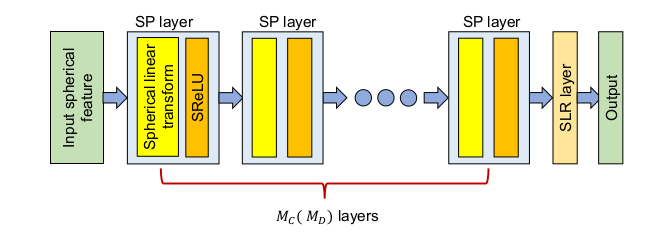
\includegraphics[width=0.7\textwidth]{Figures/From articles/sphere_layers.png}
    \caption{Spherical neural network structure}
    \label{fig: sphere_layers}
\end{figure}

Although the use of a spherical element reduces feature dimension by one, it simplifies the domain adaptation process by eliminating differences in norms. The authors define spherical adversarial training loss as follows:

\begin{equation}
    L = L_{bas}(F, C, D) + L_{rob}(F, C, \phi) + \gamma L_{ent}(F)
\end{equation}

This lost consists of three parts: basic loss, robust pseudo-label loss and conditional entropy loss. Let's start with the first one. To align features, the authors utilize basic loss which is defined as an adversarial domain adaptation loss:
\begin{equation}
L_{bas}(F, C, D) = L_{src}(F, C) + \lambda L_{adv}(F, D) + \lambda' L_{sm}(F),
\end{equation}
where $L_{src}$ is a cross-entropy loss for the source domain, $L_{adv}$ is an adversarial training loss and $L_{sm}$ is a semantic loss. The second one is conditional entropy loss which is used to keep the learned features away from the classification boundary:
\begin{equation}
L_{ent}(F) = \dfrac{1}{N_t} \sum_{j=1}^{N_t} H(C(F(x_j^t))),
\end{equation}
where $H(\cdot)$ denotes the entropy of a distribution. Additionally, the authors propose robust pseudo-label loss to increase robustness of the model. Denote $\tilde{y}_j^t = \arg \max_k [C(F(x_i^s))]_k$ as a pseudo-lebel of $x_j^t$ where $[\cdot]_k$ means the $k$-th element. To be ensured in precision of pseudo-labels, it is assumed to use new random variable $z_j \in \{0, 1\}$ for each pair $(x_j^t, \tilde{y}_j^t)$ that specify the correctness of the data (1 is correct, 0 is not). Let the probability of correct labeling be $P_\phi (z_j = 1| x_j^t, \tilde{y}_j^t)$ and $\phi$ to its parameters, then robust loss is defined as follows:

\begin{equation}
L_{rob}(F, C, \phi) = \dfrac{1}{N_0}\sum_{j=1}^{N_t} w_\phi(x_j^t) \mathcal{J}(C(F(x_j^t)), \tilde{y}_j^t),
\end{equation}
where $N_0 = \sum_{j=1}^{N_t} w_\phi(x_j^t)$ and $\mathcal{J}(\cdot, \cdot)$ is mean absolute error (MAE). The function $w_\phi (x_j^t)$ is defined using the posterior probability of correct labeling 

\begin{equation}
w_\phi(x_j^t) = \left\{\begin{split}
\gamma_j,& \;\; \text{if } \gamma_j \geq 0.5,\\
0,& \;\; \text{otherwise},
\end{split}\right.
\end{equation}
where $\gamma_j = P_\phi(z_j = 1| x_j^t, \tilde{y}_j^t)$. By utilizing a Gaussian-uniform mixture model in spherical space based on pseudo-labels, the authors model the probability $P_\phi(z_j = 1| x_j^t, \tilde{y}_j^t)$ as a function of the feature distance between the data and the center of the corresponding class. Thus, samples from target domain with a probability of correct labeling below 0.5 can be discarded. For further details of computing posterior probability, please refer to the article \cite{gu2020spherical}.  